\documentclass[a4paper]{article}
%\usepackage{simplemargins}

\usepackage[
	pdftitle={topi.link - A graph-based topology for vague geographical relations},
	pdfsubject={topi.link - A graph-based topology for vague geographical relations},
	pdfauthor={Florian Thiery},
	pdfkeywords={Linked Data, Semantic Reasoning, Vagueness, Conceptual Modeling}
]{hyperref}

% DOI and ARXIV Commands for Bib Files
% Written by Daniel Herber
% -----------------------------------------------
% one option is to use the 'note' field with this command
% -----------------------------------------------
% for example, if your doi is 10.2514/1.J052182
% then for the citation for the reference in your bib file, use
% note = "\doi{10.2514/1.J052182}",
% -----------------------------------------------
% for example, if your arxiv number is 0706.1234
% then for the citation for the reference in your bib file, use
% note = "\arxiv{0706.1234}",

% requires hyperref package for \href command
\usepackage{hyperref}

% doi command (use in bib file)
\newcommand{\doi}[1]{{doi:~\href{http://doi.org/#1}{#1}}\rmFullStop}

% arXiv command (use in bib file)
\newcommand{\arxiv}[1]{{arXiv:\href{https://arxiv.org/abs/#1}{#1}}\rmFullStop}

% command to remove full stop if the next character
\newcommand*{\rmFullStop}{\rmifnextchar{.}{}{}}

% command to check the next character and replace if present
% \rmifnextchar{X}{[removed text]}{[no X text]}
% if X is the next character, then it is removed and [removed text] is inserted
% otherwise, the character is not removed and [no X text] is inserted
% based on http://tex.stackexchange.com/questions/72827
\makeatletter
\newcommand{\rmifnextchar}[3]{%
  \begingroup
  \ltx@LocToksA{\endgroup#2}%
  \ltx@LocToksB{\endgroup#3}%
  \ltx@ifnextchar{#1}{%
    \def\next{\the\ltx@LocToksA}%
    \afterassignment\next
    \let\scratch= %
  }{%
    \the\ltx@LocToksB
  }%
}
\makeatother
%\RequirePackage{doi}
%\usepackage[square]{natbib}
\usepackage{amsmath}
\usepackage{amsfonts}
\usepackage{amssymb}
\usepackage{graphicx}

\begin{document}
\pagenumbering{gobble}

\Large
 \begin{center}
topi.link - A graph-based topology for vague geographical relations\\ 

\hspace{10pt}

% Author names and affiliations
\large
Florian Thiery$^1$$^,$$^2$\\

\hspace{10pt}

\small  
$^1$ Linked Geodesy - my private projects\\
$^2$ mainzed - Mainz Centre for Digitality in the Humanities and Cultural Studies\\
rse@fthiery.de\\

\end{center}

\normalsize

Data modelling in relational structures is a major part in geodesist's geodata modelling life. We use PostGIS databases, GeoServer applications using OGC standards, to share interoperable and open geodata via the World Wide Web. In addition, new modelling technologies allow NoSQL modelling, like graphs. Graph data is structured in nodes and edges. Geodesists know these structures if we look deeper into navigation systems technology by using the Dijkstra algorithm. 

However, to provide interoperable and semantic data, directed edge-coloured graphs, modelled in RDF using subjects, predicates and objects according to the principles of Linked (Open) Data\cite{tim_linked_2006} are necessary. LOD are already widely used in geodesy\cite{hart_linked_2013}: e.g. GeoSPARQL\cite{battle_geosparql_2011}, LinkedGeoData\cite{auer_linkedgeodata_2009} and Britain’s Ordnance Survey\cite{shadbolt_linked_2012}.

But what can we do if our data only consists of toponyms which have geographical relations without coordinate information? We could model these spatial relations\cite{clementini_modelling_1994} using the common DE-9IM\cite{mark_modeling_1994} topological model; but in reality this nine relations are not enough. Moreover, these relations are very vague. Furthermore, inference making, e.g. for the property \textit{northOf}\cite{thiery_zenodo_1}, via reasoning\cite{thiery_zenodo_4}, to create new knowledge, would be very cool: we need a 'little minion' to all this stuff.

For modelling these kinds of vague geographical graph data, the Academic Meta Tool\cite{unold_academic_2019} (AMT) can be used: this paper focuses on prototypical examples of the 'topi Ontology'\cite{thiery_zenodo_2} by introducing AMT modelling strategies, the AMT JavaScript framework\cite{thiery_zenodo_3} and the topi.link playground\cite{thiery_topilink_2019}.


\begin{figure}[!htb]
	\centering
		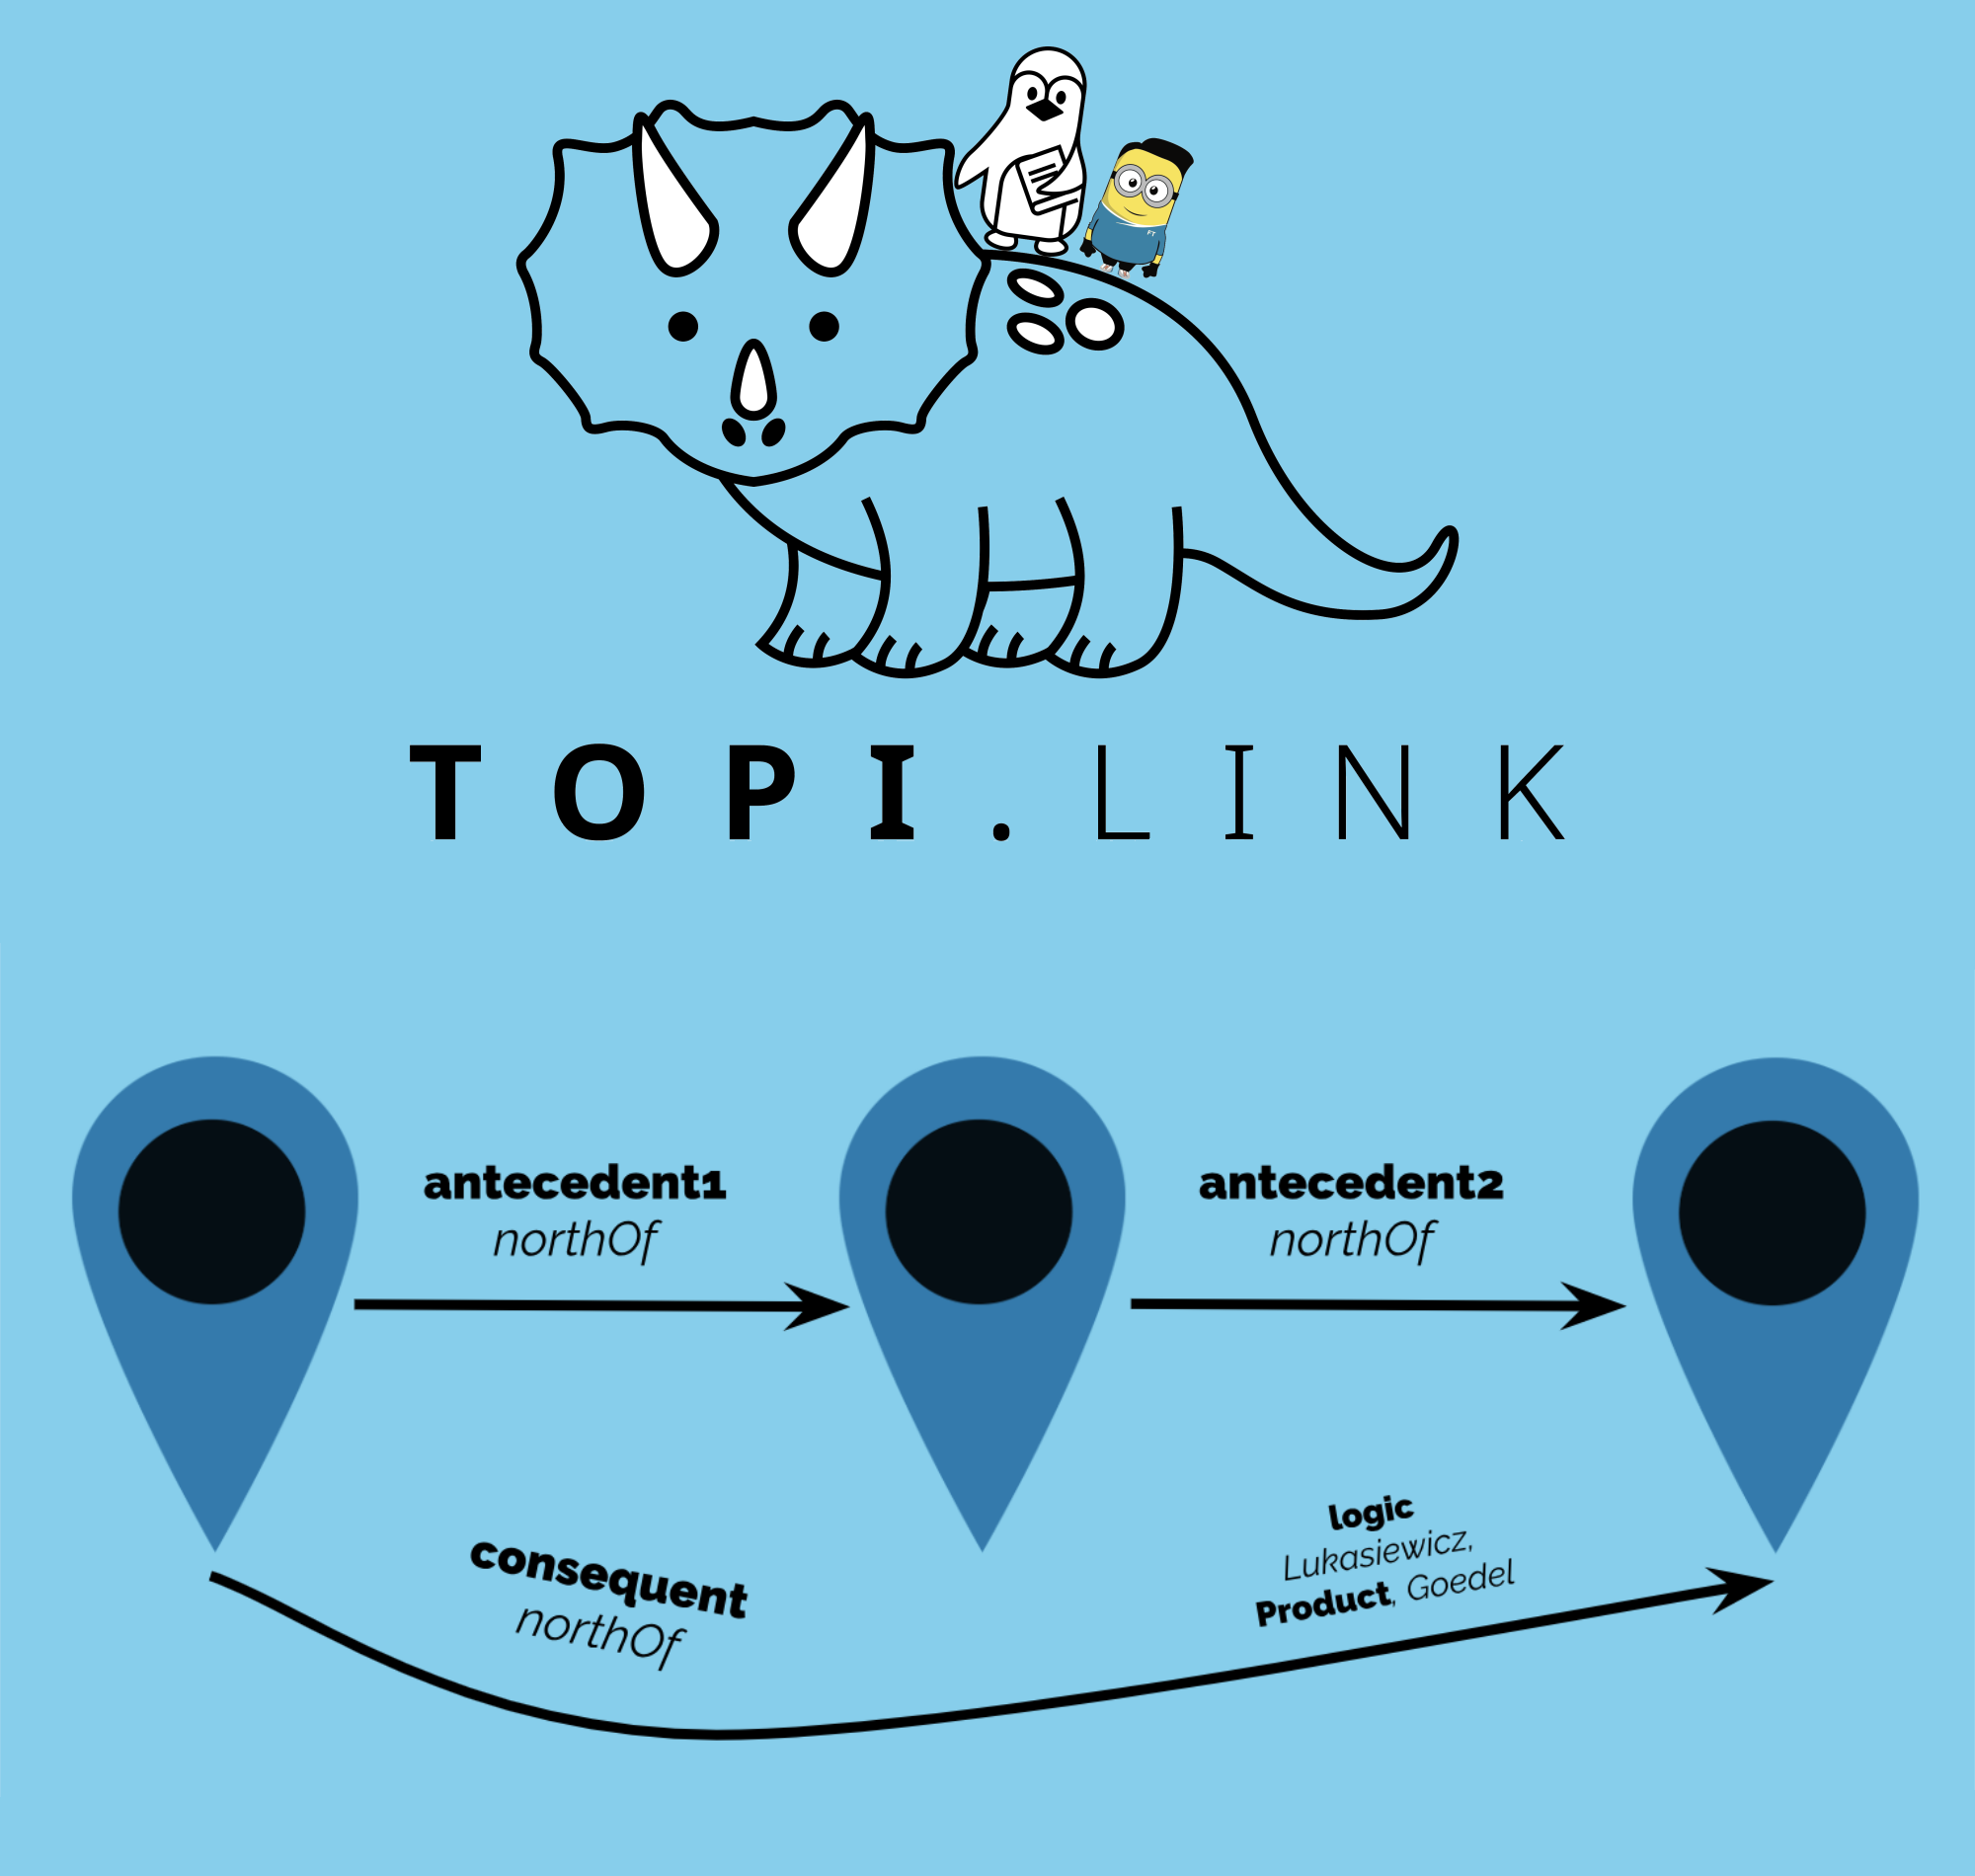
\includegraphics[width=0.50\textwidth]{D:/src/igsm2019-topi/pic.png}
	\caption{topi.link scheme}
	\label{topilinkscheme}
\end{figure}

\bibliographystyle{IEEEtran}
\bibliography{bib}

\end{document}